\chapter{評価}
\label{evaluation}

本章では第4章の\ref{implementation}で設定した3つの実験の結果及び考察を行う。

実験1の結果\label{evo1}では\ref{exp1}で示した設定もとに実験を行い、その結果を述べ各データセットにおいてどの程度の学習性能を示したか結論を述べる。
実験2の結果\label{evo2}では\ref{exp2}で示した設定もとに実験を行い、\ref{af-class}の表を軸にどのような活性化関数になったか、損失を見ながら考察を行い結論を述べる。
実験3の結果\label{evo3}では\ref{exp3}で示した設定もとに実験を行い、一般的にどのような条件でK-AFがより良い性能を出すか、また、欠点が存在するか調査する。

\label{result}では各実験による考察結果から、\ref{kadai}に対してどの程度K-AFが性能を示すことができたか分析を行う。
そして最後に第6章への結論\ref{conclusion}へと導く。


\section{実験1の結果 既存の活性化関数との比較実験}
\label{evo1}
\ref{exp1}で示した比較実験の結果を記述する。

\subsection{irisでの比較実験}
\label{ev:iris}

第4章の\ref{impl:iris}で設定した実験を行い、結果を以下にまとめた。
\subsubsection{設定1及び設定2の結果と考察}


\begin{table}[htbp]
    \begin{center}
        \caption{irisの設定1及び設定2のAccuracy}
        \vspace{2mm} 
        \begin{tabular}{l*{2}{c}r}
            活性化関数  & 設定1のAccuracy &  設定2のAccuracy \\
            \hline
            K-AF            & 72.0 & 26.0 \\
            Sigmoid            & 68.0 & 77.3\\
            Linear            & 20.0 & 53.0\\
            ReLU        &  49.6 &  38.3\\
            Swish           & 87.3 & 47.3 \\
            Mish           & 60.0 & 65.0 \\
    
        \end{tabular}
    \end{center}
\end{table}


\subsubsection{設定1及び設定2のLossTrainig}
\label{iris:loss}



\begin{figure}[hbtp]
    \begin{center}
        \begin{tabular}{c}
            \begin{minipage}{0.5\hsize}
                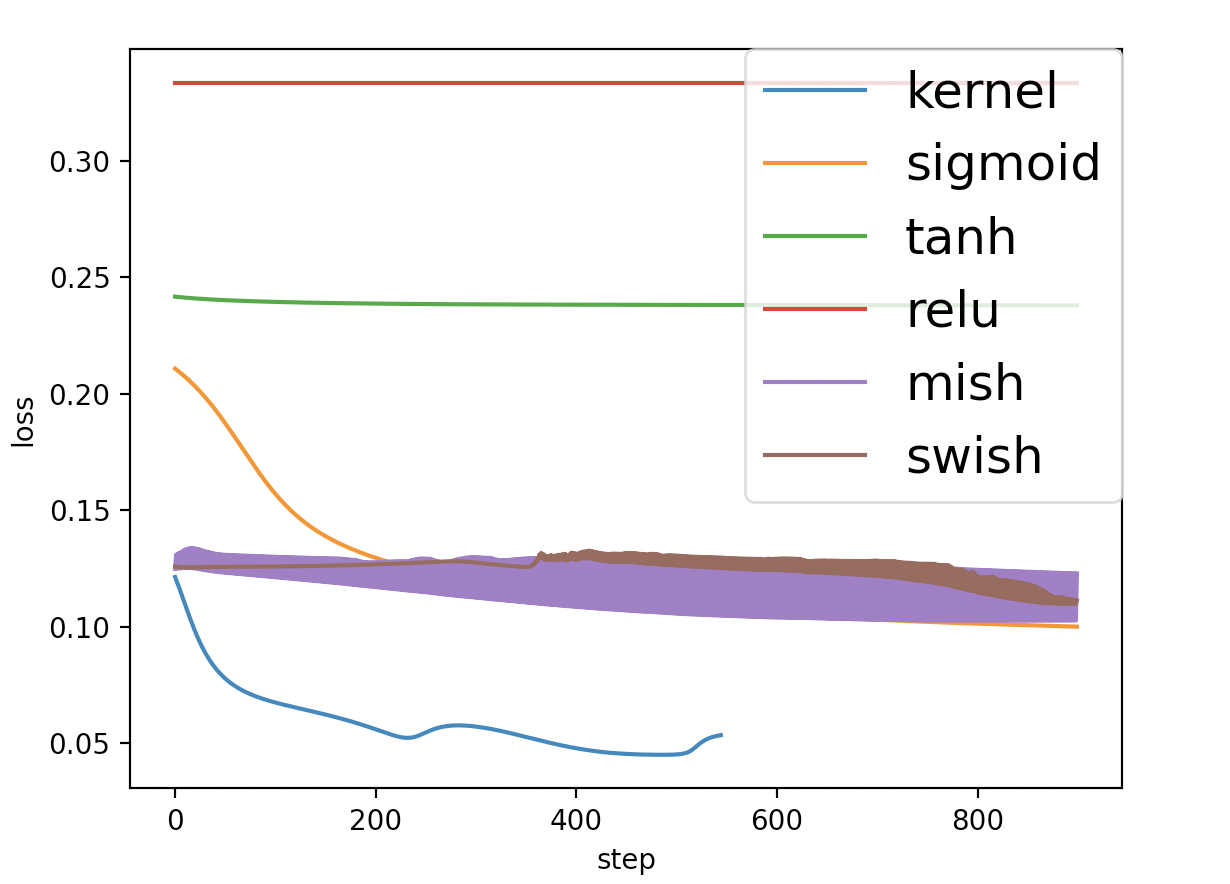
\includegraphics[clip, width=7cm]{asset/iris_0.1_1000_3_02_sgd_non_kaiming_uniform.png}
                    \caption{irisの設定1の結果のLossTraining}
                    \label{iris_1}
            \end{minipage}
            \hspace{10pt}
            \begin{minipage}{0.5\hsize}
                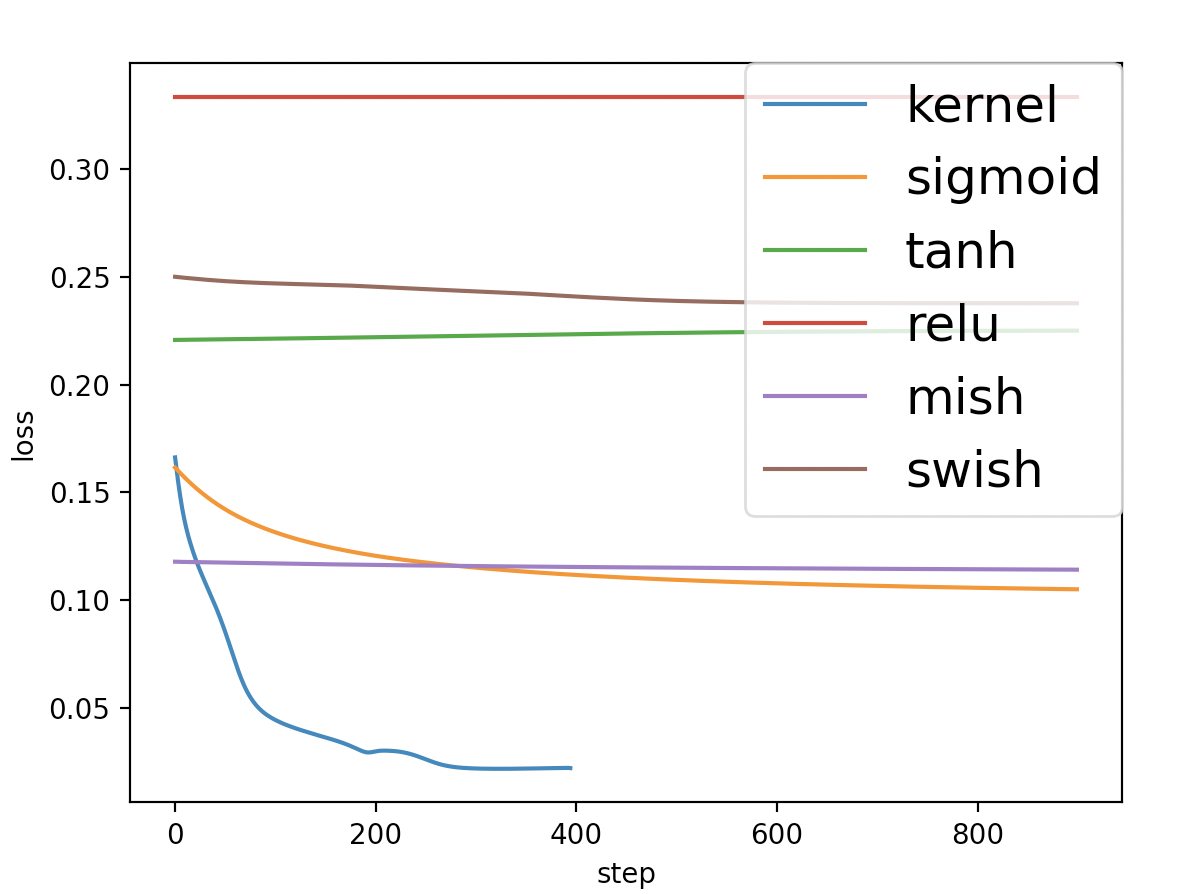
\includegraphics[clip, width=7cm]{asset/iris_0.1_1000_3_02_sgd_l2_kaiming_uniform.png}
                    \caption{irisの設定2の結果のLossTraining}
                    \label{iris_2}
            \end{minipage}
        \end{tabular}
    \end{center}
\end{figure}


\subsubsection{irisでの実験結果の考察}


irisは最も単純な分類問題の一つであるが結果\ref{iris:result}を見るに特に学習を効率的にするテクニックを使わない場合は良い精度が出せている。
Swishが高い性能を出していることもわかる。
また、L2のRegularizerを入れるとかなり精度が下がってしまうことから、K-AFは既存の学習テクニックとの組み合わせでは精度が向上しないことがわかる。






\subsection{digitsでの比較実験}
\label{ev:digitsでの比較実験}
第4章の\ref{impl:digits}で設定した実験を行い、結果を以下にまとめた。
\subsubsection{設定1及び設定2の結果}
\label{digits:result}

\begin{table}[htbp]
    \begin{center}
        \caption{digitsの設定1及び設定2のAccuracy}
        \vspace{2mm} 
        \begin{tabular}{l*{2}{c}r}
            活性化関数              & 設定1のAccuracy &  設定2のAccuracy \\
            \hline
            K-AF            & 91.6 & 60.0 \\
            Sigmoid            & 92.0 & 68.6\\
            Tanh            & 95.6 & 89.6 \\
            ReLU        & 38.0 & 54.3 \\
            Swish           & 50.3 & 56.6 \\
            Mish           & 55.6 & 53.3 \\
    
        \end{tabular}
    \end{center}
\end{table}


\subsubsection{設定1及び設定2のLossTrainig}
\label{digits:loss}



\begin{figure}[hbtp]
    \begin{center}
        \begin{tabular}{c}
            \begin{minipage}{0.5\hsize}
                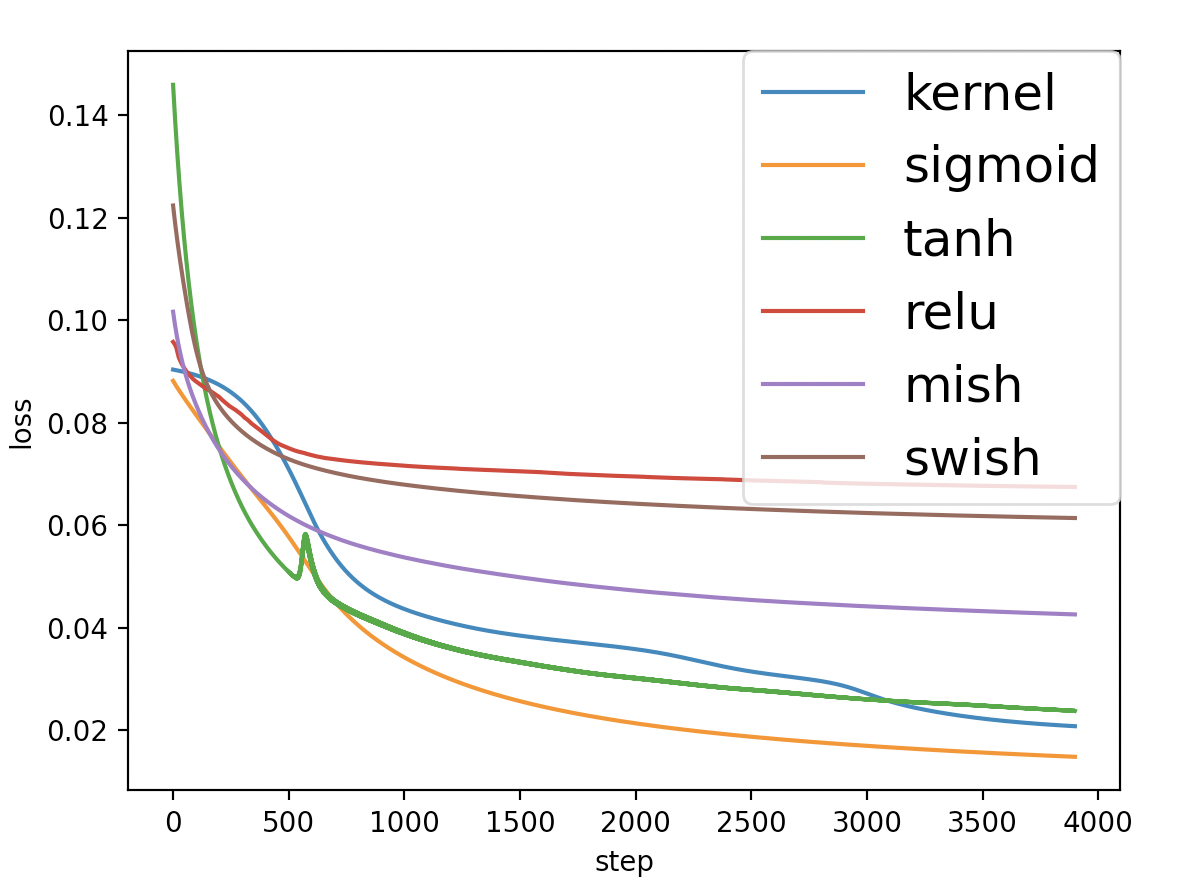
\includegraphics[clip, width=7cm]{asset/digits_0.01_4000_3_002_sgd_non_kaiming_uniform.png}
                    \caption{digitsの設定1の結果のLossTraining}
                    \label{digits_1}
            \end{minipage}
            \hspace{10pt}
            \begin{minipage}{0.5\hsize}
                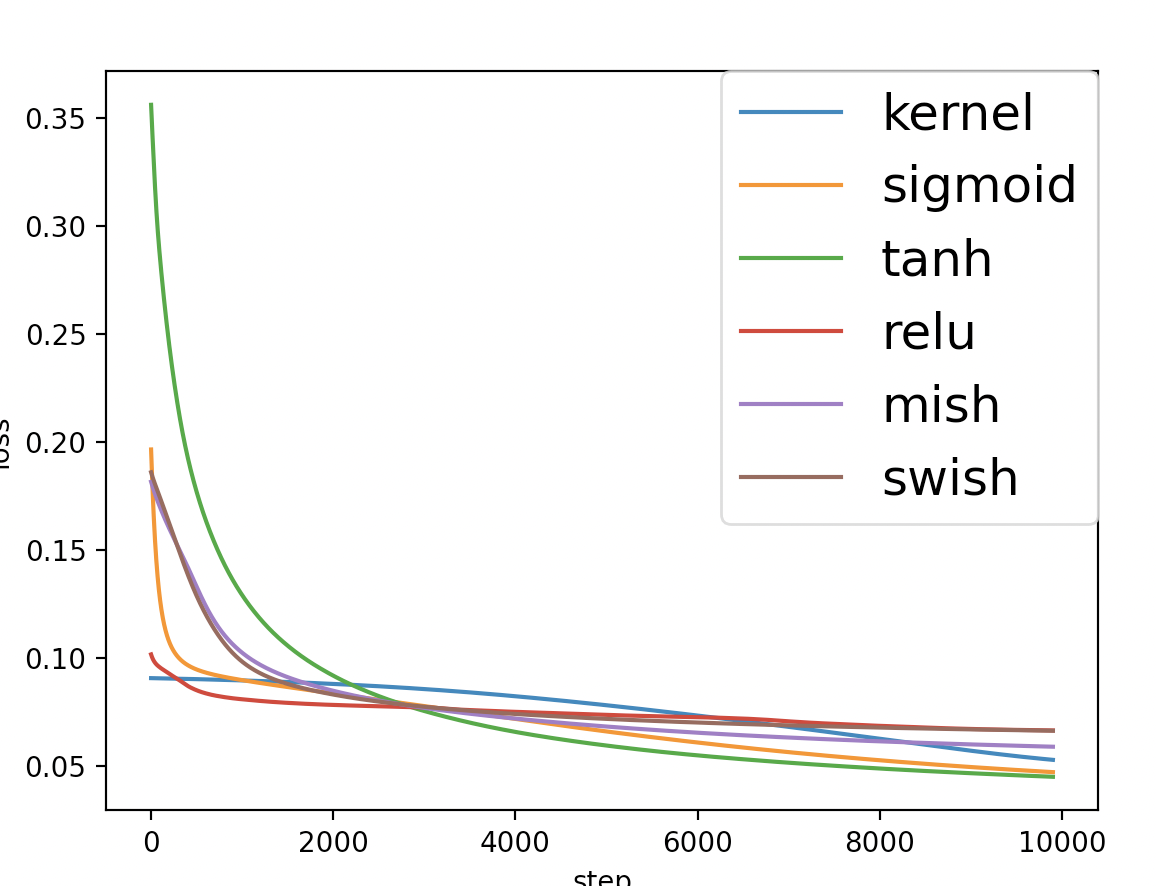
\includegraphics[clip, width=7cm]{asset/digits_0.001_10000_3_002_adam_non_kaiming_uniform.png}
                    \caption{digitsの設定2の結果のLossTraining}
                    \label{digits_2}
            \end{minipage}
        \end{tabular}
    \end{center}
\end{figure}


\subsubsection{digitsでの実験結果の考察}
結果\ref{digits:result}を見ると設定1の場合では91.6\%とSigmoidやTanhといったラベリングによく用いられる活性化関数に匹敵する精度を出せた。ReLU、Mish、Swish等のの上限値が存在しない関数よりも遥かに良い性能を出すことができた。
設定2の場合でもSigmoidやTanhほどの成果は出なかったものの、上限値が存在しない関数よりはいい性能を出すことができた。

TrainigLossのグラフ\ref{digits:result}を見ると、設定の1,2共に順調に下に推移してることがわかる。
設定1の方で途中でTanhを追い抜いている理由は、活性化関数の形が急激に変わる瞬間があるからである。


\subsection{wineでの実験と設定}
\label{ev:wineでの実験と設定}

第4章の\ref{impl:wine}で設定した実験を行い、結果を以下にまとめた。
\subsubsection{設定1及び設定2の結果と考察}


\begin{table}[htbp]
    \begin{center}
        \caption{wineの設定1及び設定2の結果Accuracy}
        \vspace{2mm} 
        \begin{tabular}{l*{2}{c}r}
            活性化関数              & 設定1のAccuracy &  設定2のAccuracy \\
            \hline
            K-AF            & 72.0 & 27.0 \\
            Sigmoid            & 33.3 & 43.0\\
            Linear            & 33.3 & 38.3\\
            ReLU        & 33.3 & 0.0\\
            Swish           & 33.3 & 27 \\
            Mish           & 33.3 &  27.0\\
    
        \end{tabular}
    \end{center}
\end{table}


\subsubsection{設定1及び設定2のLossTrainig}
\label{digits:loss}

\begin{figure}[hbtp]
    \begin{center}
        \begin{tabular}{c}
            \begin{minipage}{0.5\hsize}
                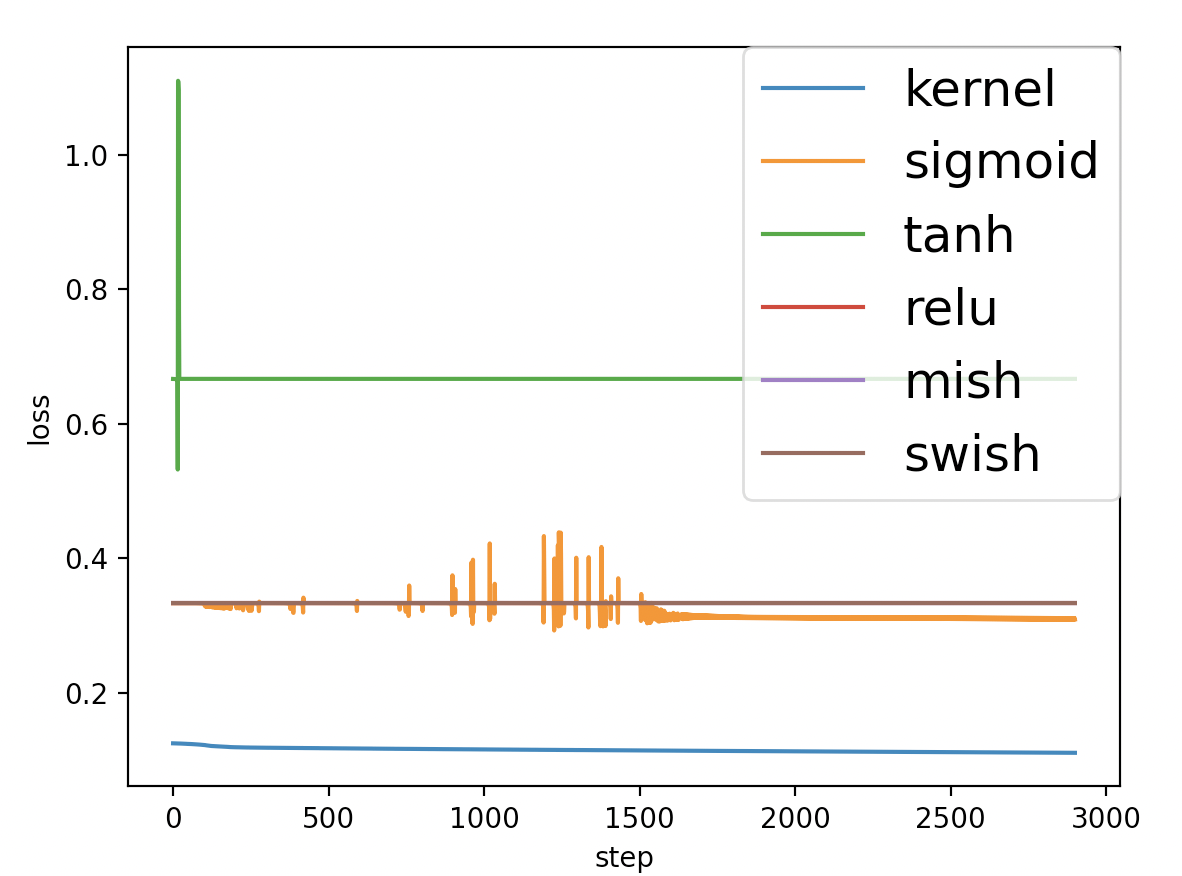
\includegraphics[clip, width=7cm]{asset/wine_0.001_3000_3_015_sgd_non_kaiming_uniform.png}
                    \caption{wineの設定1の結果のLossTraining}
                    \label{wine_1}
            \end{minipage}
            \hspace{10pt}
            \begin{minipage}{0.5\hsize}
                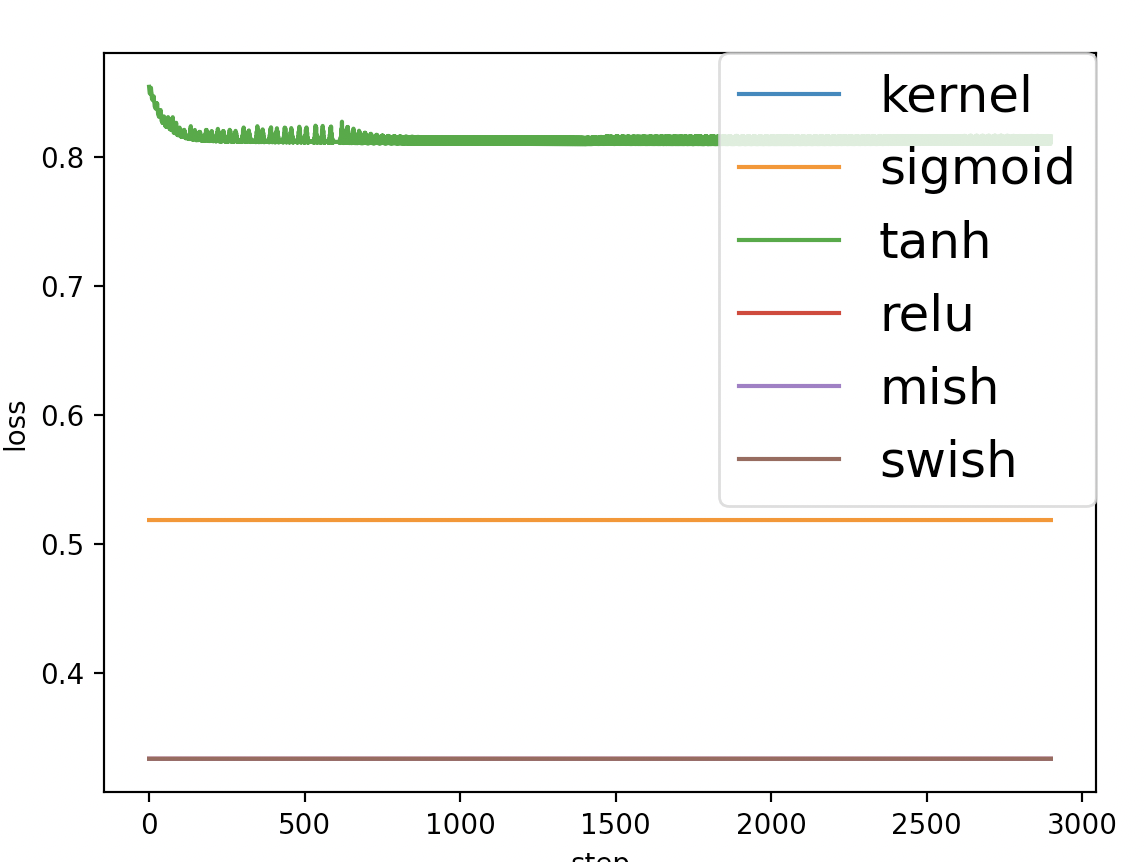
\includegraphics[clip, width=7cm]{asset/wine_0.001_3000_3_015_adam_non_kaiming_uniform}
                    \caption{wineの設定2の結果のLossTraining}
                    \label{wine_2}
            \end{minipage}
        \end{tabular}
    \end{center}
\end{figure}


\subsubsection{wineでの実験結果の考察}
結果\ref{wine:result}を見るとwineはもともと決定木に使用されるデータセットのためか、設定1ではK-AF以外では発散してしまっていることがわかる。
また、設定2はoptimizerをadamに変えただけ、学習が失敗することがわかった。
全体を通してもSGDのK-AFが最大のAccuracyを叩き出している。







\subsection{bostonでの比較実験}
\label{ev:bostonでの比較実験}

第4章の\ref{impl:boston}で設定した実験を行い、結果を以下にまとめた。
\subsubsection{設定1及び設定2の結果と考察}


\begin{table}[htbp]
    \begin{center}
        \caption{bostonの設定1及び設定2のAccuracy}
        \vspace{2mm} 
        \begin{tabular}{l*{2}{c}r}
            活性化関数              & 設定1のMSE &  設定2のMSE \\
            \hline
            K-AF            & 49.4 & 69.4 \\
            Sigmoid            & 523.0 & 541.4 \\
            Tanh            & 540.6 &  567.8 \\
            ReLU        & 359.2 & 473.4 \\
            Swish           & 257.0 & 372.4 \\
            Mish           & 360.0 & 472.4 \\
    
        \end{tabular}
    \end{center}
\end{table}


\subsubsection{設定1及び設定2のLossTrainig}
\label{boston:loss}

\begin{figure}[hbtp]
    \begin{center}
        \begin{tabular}{c}
            \begin{minipage}{0.5\hsize}
                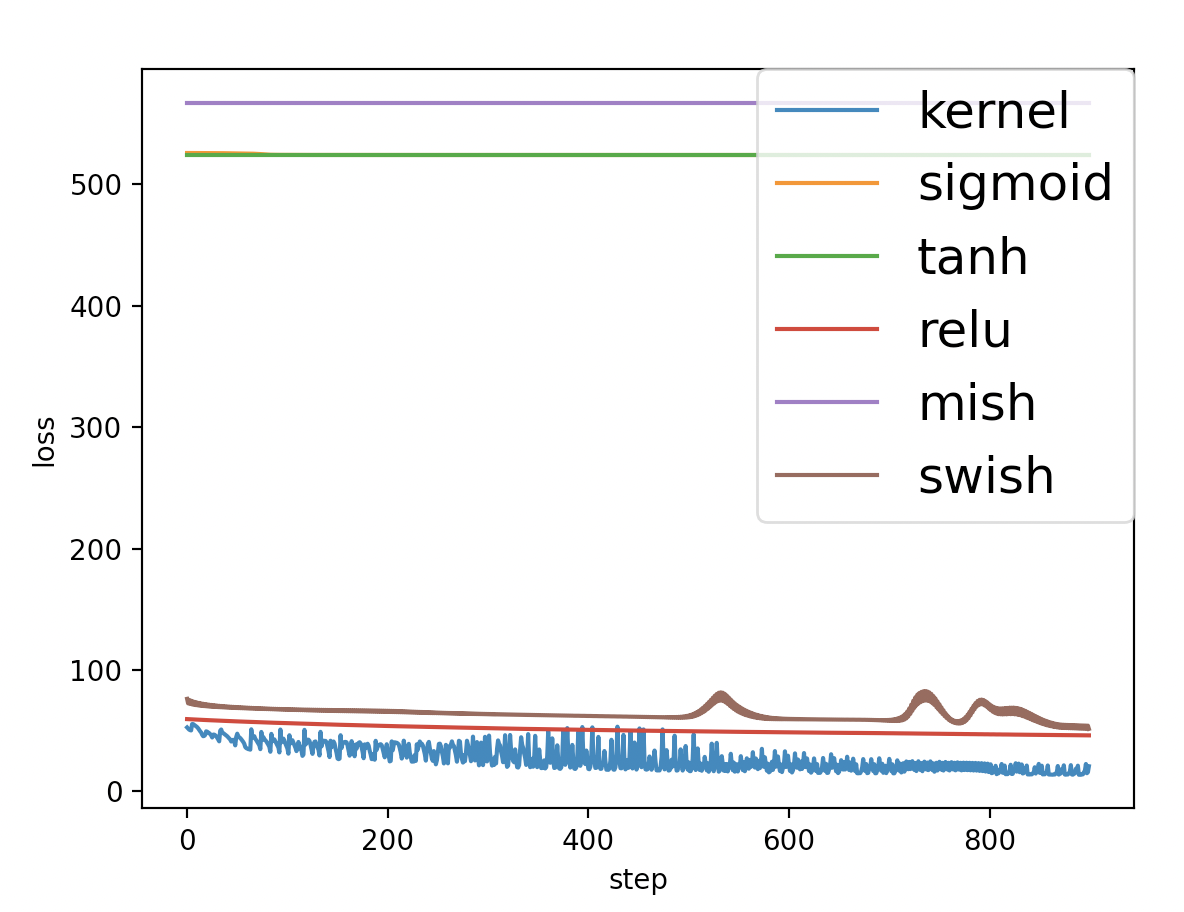
\includegraphics[clip, width=7cm]{asset/boston_0.00001_1000_3_005_sgd_non_kaiming_uniform.png}
                    \caption{bostonの設定1の結果のLossTraining}
                    \label{boston_1}
            \end{minipage}
            \hspace{10pt}
            \begin{minipage}{0.5\hsize}
                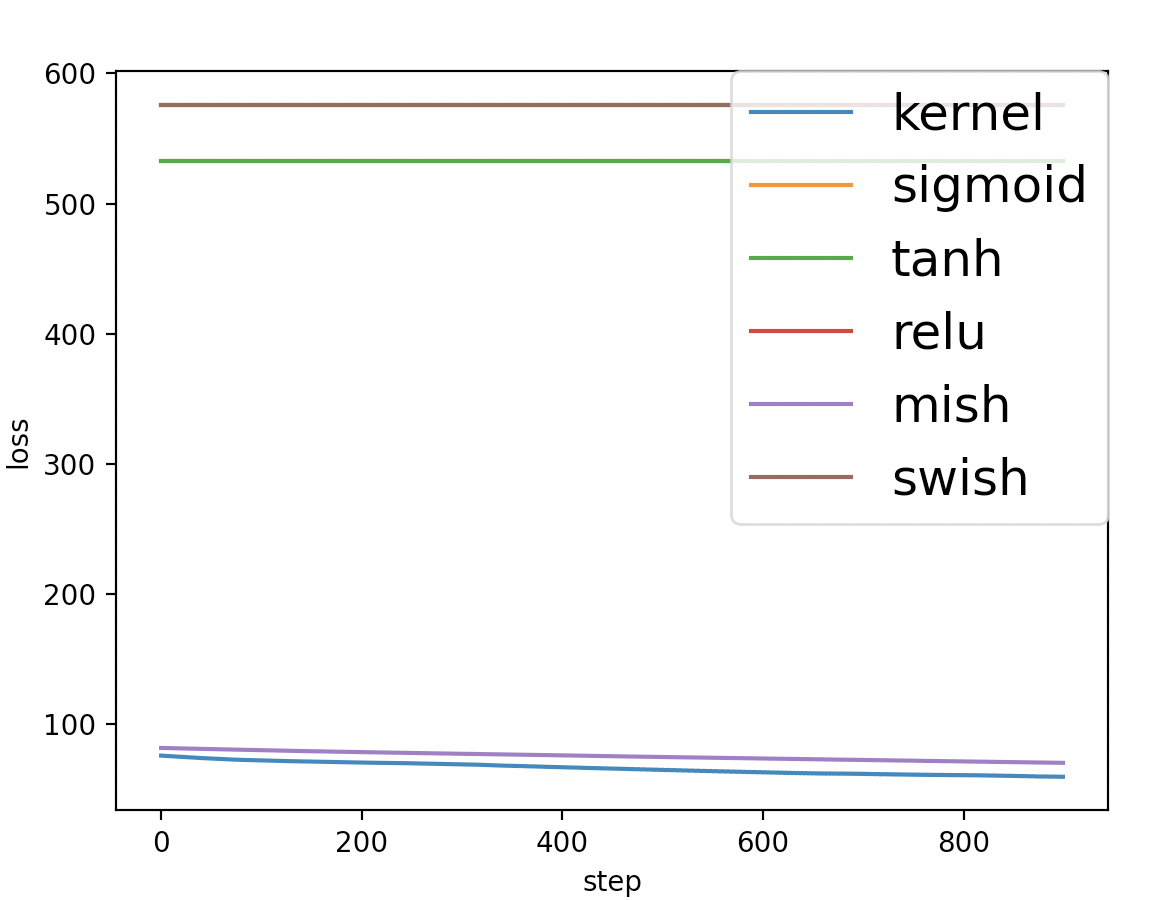
\includegraphics[clip, width=7cm]{asset/boston_0.00001_1000_3_005_sgd_non_xavier_uniform.png}
                    \caption{bostonの設定2の結果のLossTraining}
                    \label{boston_2}
            \end{minipage}
        \end{tabular}
    \end{center}
\end{figure}


\subsubsection{bostonでの実験結果の考察}
bostonは本実験で唯一の回帰のデータセットである。
結果\ref{boston:result}を見るに、SigomoidとTanhは上限値のある関数のため、うまくいかないことは容易に想像がつくが、ReLU等の関数よりも高い精度が出ることがわかった。





\subsection{breast\_cancerでの比較実験}
\label{ev:breastcancer}

\subsubsection{設定1及び設定2の結果と考察}


\begin{table}[htbp]
    \begin{center}
        \caption{breast\_cancerの設定1及び設定2のAccuracy}
        \vspace{2mm} 
        \begin{tabular}{l*{2}{c}r}
            活性化関数              & 設定1のAccuracy &  設定2のAccuracy \\
            \hline
            K-AF            & 43.0 & 90.3 \\
            Sigmoid            & 47.3 & 78.3\\
            Linear            & 60.0 & 29.0\\
            ReLU        & 43.0 & 29.0\\
            Swish           & 55.3 & 42.6\\
            Mish           & 47.3 & 42.6\\
    
        \end{tabular}
    \end{center}
\end{table}




\subsubsection{設定1及び設定2のLossTrainig}
\label{breastcancer:loss}

\begin{figure}[hbtp]
    \begin{center}
        \begin{tabular}{c}
            \begin{minipage}{0.5\hsize}
                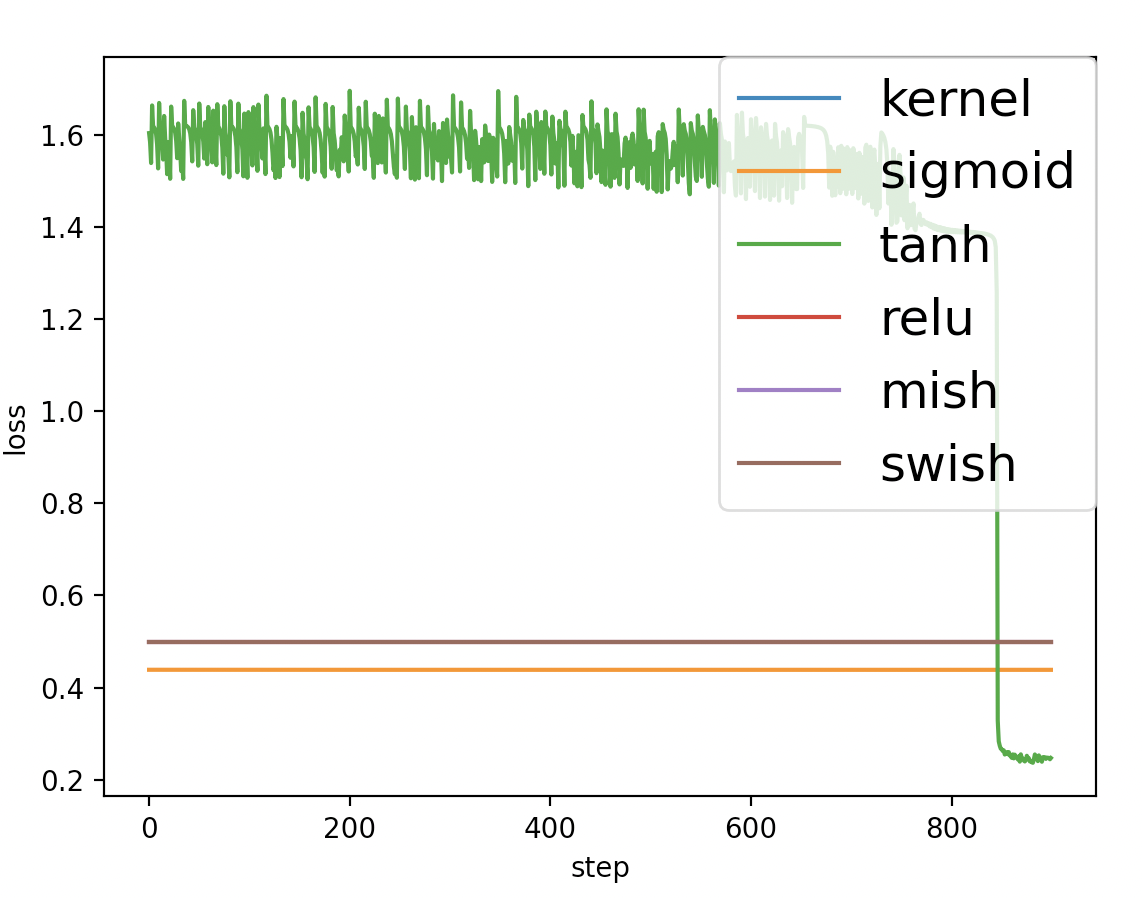
\includegraphics[clip, width=7cm]{asset/breastcancer_0.001_1000_3_005_sgd_non_kaiming_uniform}
                    \caption{breastcancerの設定1の結果のLossTraining}
                    \label{breastcancer_1}
            \end{minipage}
            \hspace{10pt}
            \begin{minipage}{0.5\hsize}
                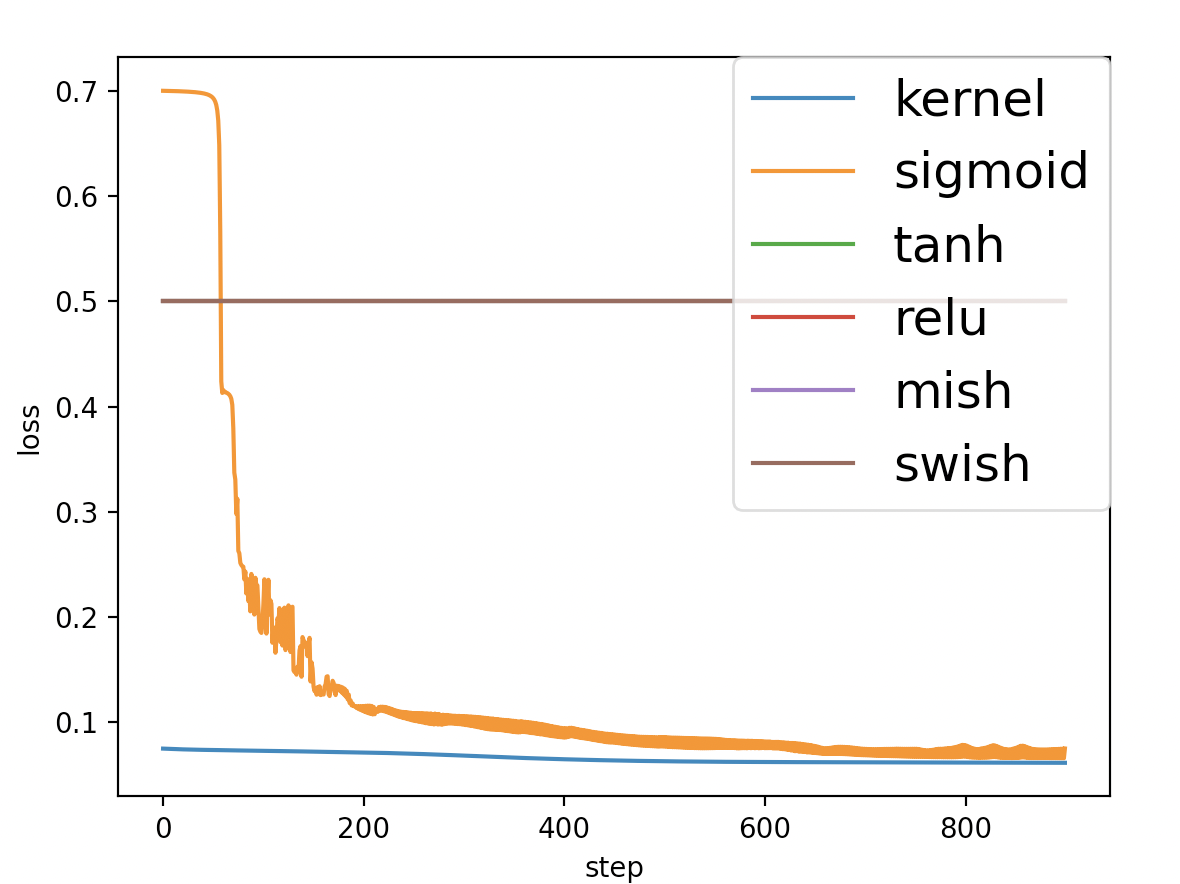
\includegraphics[clip, width=7cm]{asset/breastcancer_0.001_1000_3_05_sgd_non_kaiming_uniform}
                    \caption{breastcancerの設定2の結果のLossTraining}
                    \label{breastcancer_2}
            \end{minipage}
        \end{tabular}
    \end{center}
\end{figure}


\subsubsection{breastcancerでの実験結果の考察}
結果\ref{breastcancer:result}を見るに、カーネル密度関数を推定するためのデータセットに依存して、発散することとそうではない場合があるようである。
こちらも決定木の性能評価でよく疲れるデータセットであるため、ニューラルネットワークで評価をするのには向いていないことが精度が出づらいことの原因であると考えられる。


\subsection{実験1全体のまとめ}
結果全体を見ると、K-AFは本実験で使うようなデータセットの場合でも、いい条件で学習することができれば
かなり高い精度でどのデータセットも学習できることがわかる。
特に決定木の問題に対してもcalc\_numを多めに取ることができれば予想以上に高い精度を出すことがわかった。


\section{実験2の結果 K-AFの関数形状の調査}
\label{evo2}
\ref{exp2}で示した比較実験の結果を記述する。





\subsubsection{irisの活性化関数}
実験の設定は表\ref{dataset_name}のLearningRateと表\ref{exp:iris}のLR以外の設定を用いる。
推論した活性化関数の形は図\ref{infer_iris}のようになる。
\begin{figure}[hbtp]
    \begin{center}
        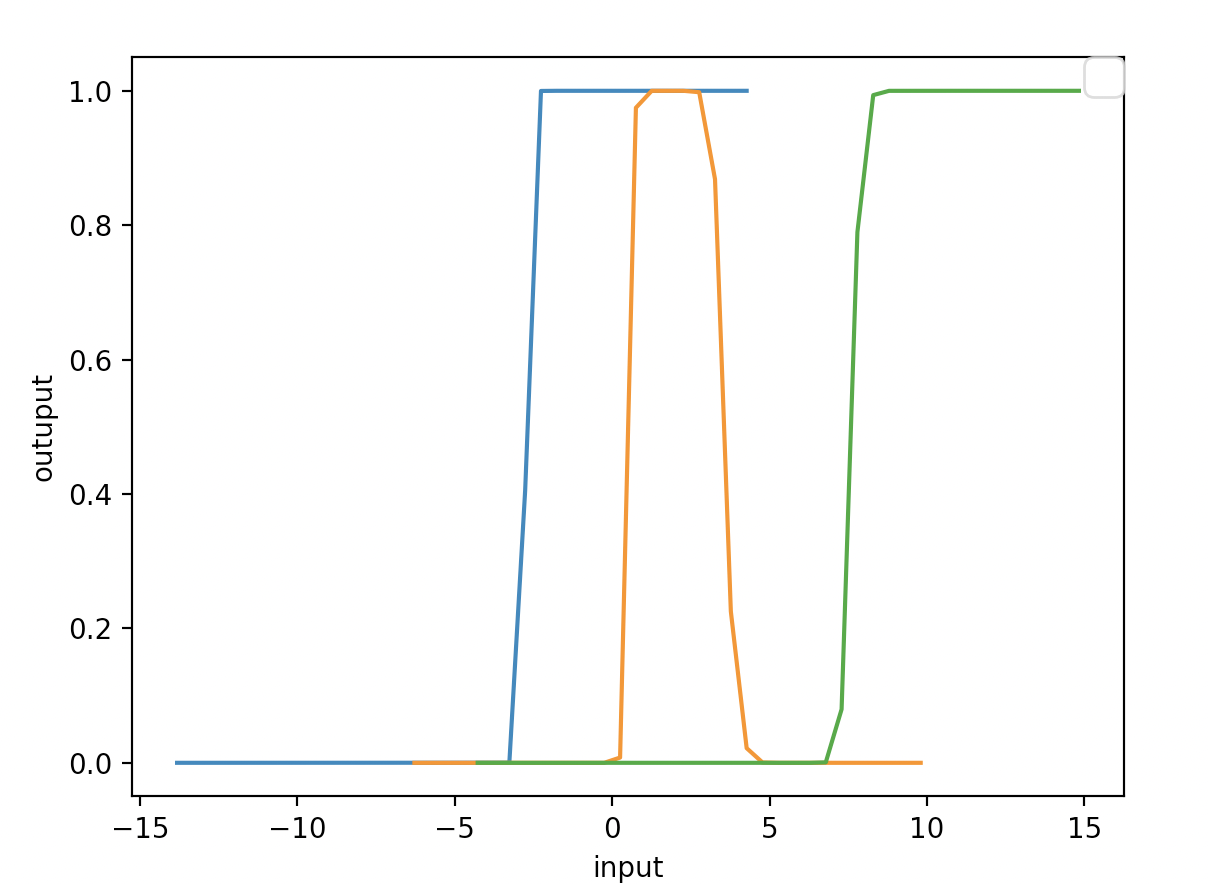
\includegraphics[width=10cm]{asset/iris-0.1.png}
            \caption{irisで推論した活性化関数の形}
            \label{ifer_iris}
    \end{center}
\end{figure}

またこれを\ref{af-class}の表に埋めると表\ref{anal_iris}のようになる。
\begin{table}[htbp]
    \begin{center}
        \caption{irisで推論した活性化関数の分析表}
        \label{anal_iris}
        \vspace{2mm} 
        \begin{tabular}{ |c|c|c| }
        単調増加関数か & 勾配が$ 0 $の点があるか & 上限値があるか   \\
        \hline
        × & ○ & ○   \\
        \end{tabular}
    \end{center}
\end{table}



単純な分類問題であるが、\ref{ifer_iris}を観察するにSigmoid等の活性化関数と違い単調増加もしくは単調減少しない活性化関数が導かれることがわかった。




\subsubsection{digitsの活性化関数}
実験の設定は表\ref{dataset_name}のLearningRateと表\ref{exp:digits}のLR以外の設定を用いる。
推論した活性化関数の形は図\ref{infer_digits}のようになる。
\begin{figure}[hbtp]
    \begin{center}
        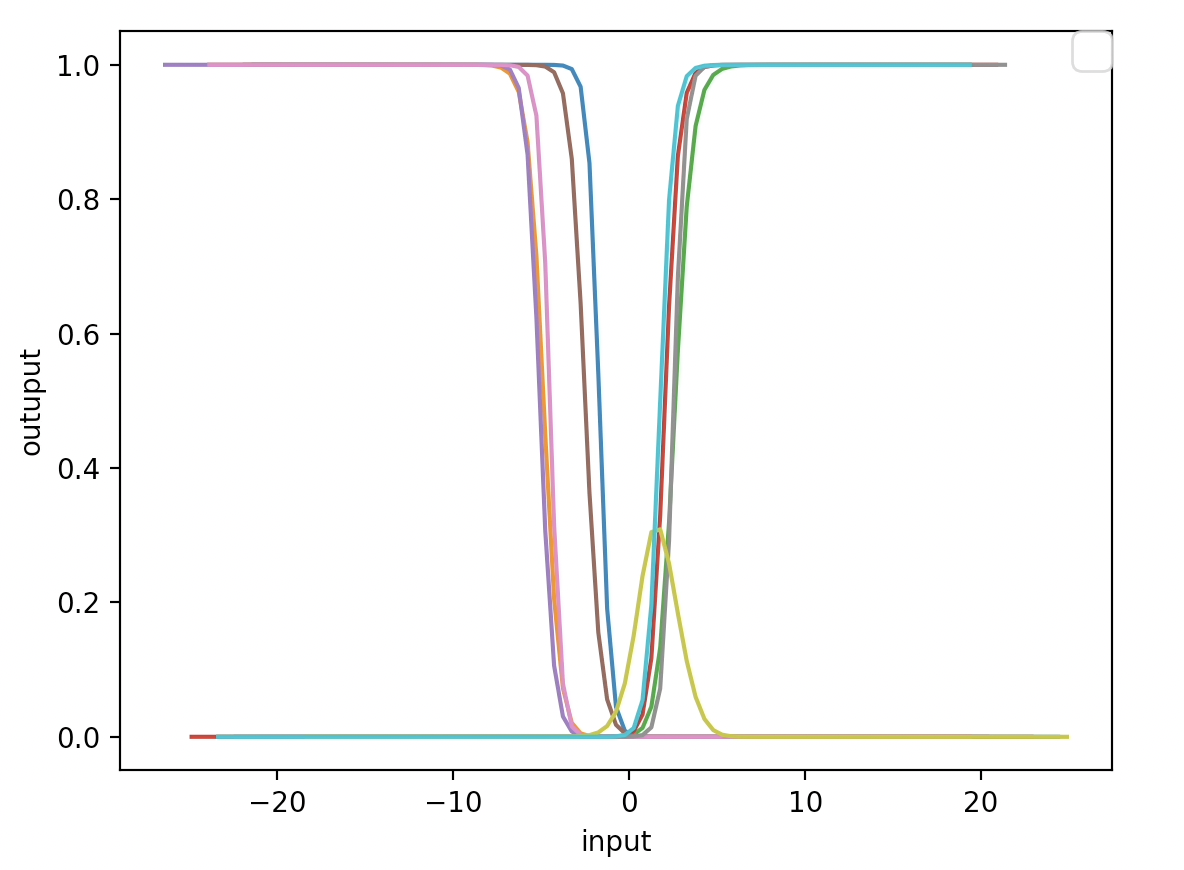
\includegraphics[width=10cm]{asset/digits-0.1.png}
            \caption{digitsで推論した活性化関数の形}
            \label{ifer_digits}
    \end{center}
\end{figure}

またこれを\ref{af-class}の表に埋めると表\ref{anal_digits}のようになる。
\begin{table}[htbp]
    \begin{center}
        \caption{digitsで推論した活性化関数の分析表}
        \label{anal_digits}
        \vspace{2mm} 
        \begin{tabular}{ |c|c|c| }
        単調増加関数か & 勾配が$ 0 $の点があるか & 上限値があるか   \\
        \hline
        ▲ & ○ & ○   \\
        \end{tabular}
    \end{center}
\end{table}

▲になる理由は単調増加とは対象的な単調減少の関数も推論した関数の中に存在するからである。
推論するデータセットがラベリング問題であるため上限値が$ 1 $であることから、このような形になったと考えられる。
例外的に一つ形が崩れているが、Sigmoidと関数の形がにているため、使用する関数としてもSigmoidのような形のもので十分な精度が出ることが予想できる。
実際に\ref{ev:wineでの実験と設定}ではSigmoidやTanhでも十分な性能を出している。





\subsubsection{wineの活性化関数}
実験の設定は表\ref{dataset_name}のLearningRateと表\ref{exp:wine}のLR以外の設定を用いる。
推論した活性化関数の形は図\ref{infer_wine}のようになる。
\begin{figure}[hbtp]
    \begin{center}
        \includegraphics[width=10cm]{asset/wine-0.1.png}
            \caption{wineで推論した活性化関数の形}
            \label{ifer_wine}
    \end{center}
\end{figure}

またこれを\ref{af-class}の表に埋めると表\ref{anal_wine}のようになる。
\begin{table}[htbp]
    \begin{center}
        \caption{wineで推論した活性化関数の分析表}
        \label{anal_wine}
        \vspace{2mm} 
        \begin{tabular}{ |c|c|c| }
        単調増加関数か & 勾配が$ 0 $の点があるか & 上限値があるか   \\
        \hline
        ▲ & ○ & ○   \\
        \end{tabular}
    \end{center}
\end{table}



















\section{実験3の結果 K-AFの性能が上がる条件探査}
\label{evo3}
\ref{exp3}で示した比較実験の結果を記述する。
wine及びbostonのデータセットで最も性能が良かったニューラルネットワークの設定のトップ5を記述する。

\subsubsection{wineの場合}

\begin{table}[htbp]
    \begin{center}
        \caption{wineを推論するときの最もいい設定}
        \label{winebest}
        \vspace{2mm} 
        \begin{tabular}{ |c|c|c| }
        組み合わせ & Acc & エラーの回数 \\
        \hline
        iris           & $ 10^{-3} $    & 3 \\
        digits         & $ 10^{-3} $    & 3 \\
        wine           & $ 10^{-3} $    & 3 \\
        boston         & $ 10^{-3} $    & 13  \\
        breast\_cancer & $ 10^{-3} $    & 30 \\
        \end{tabular}
    \end{center}
\end{table}

表\ref{winebest}を参考にすると

\subsubsection{bostonの場合}

\begin{table}[htbp]
    \begin{center}
        \caption{bostonを推論するときの最もいい設定}
        \label{bostonbest}
        \vspace{2mm} 
        \begin{tabular}{ |c|c|c| }
        組み合わせ & Acc & エラーの回数 \\
        \hline
        iris           & $ 10^{-3} $    & 3 \\
        digits         & $ 10^{-3} $    & 3 \\
        wine           & $ 10^{-3} $    & 3 \\
        boston         & $ 10^{-3} $    & 13  \\
        breast\_cancer & $ 10^{-3} $    & 30 \\
        \end{tabular}
    \end{center}
\end{table}




\subsection{性能評価まとめ}
wineとbostonの結果をまとめるとと言うことがわかった。


\section{まとめ}

K-AFの精度、勾配消失の有無、実用性の観点から先行研究との比較を行った。
実験結果を踏まえ, 第 6 章で解決した課題をまとめ、将来への展望を述べる。


%%% Local Variables:
%%% mode: japanese-latex
%%% TeX-master: "./thesis"
%%% End:
